

\documentclass{beamer}
 
\usepackage[utf8]{inputenc}
 \usetheme{Madrid}
 \usecolortheme{beaver}
 \usefonttheme{structuresmallcapsserif}
 \usepackage{listings}
%Information to be included in the title page:


\title[CORBA] %optional
{Corba}

\subtitle{An Overview}

\author[Dr. Joseph Kehoe] % (optional, for multiple authors)
{Joseph Kehoe\inst{1}}

\institute[IT Carlow] % (optional)
{
	\inst{1}%
	Department of Computing and Networking\\
	Institute of Technology Carlow
}

\date[ITC 2018] % (optional)
{CDD101, 2018}

\logo{
\includegraphics[height=1.5cm]{../../itcarlowlogo.png}}




 
 \AtBeginSection[]
 {
 	\begin{frame}
 		\frametitle{Table of Contents}
 		\tableofcontents[currentsection]
 	\end{frame}
 }
 
 
 
\begin{document}
 
\frame{\titlepage}
 
%  \begin{frame}
%  	\frametitle{Table of Contents}
%  	\tableofcontents
%  \end{frame}
 


  \begin{frame}
  	\frametitle{Introduction}

  	\begin{itemize}
  		\item Common Object Request Broker Architecture
  		\item Open Standard Managed by the Object Management Group (OMG)
  		\item Ratified by ISO
  		\item Set up to create an open standard for distributed object interaction
  		\item CORBA enables collaboration between systems on different operating systems, programming languages, and computing hardware
  		\item CORBA uses an object-oriented model although the systems that use the CORBA do not have to be object-oriented
  	\end{itemize}

  	
  		%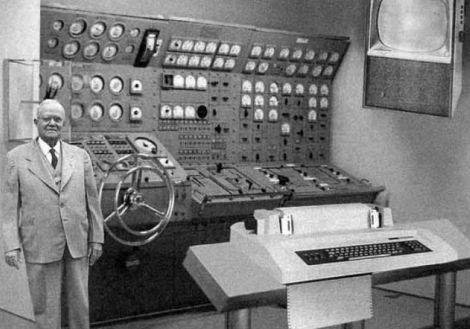
\includegraphics[height=4cm]{Old-Server.jpg}
  \end{frame}
  
    \begin{frame}
    	\frametitle{Corba}
    	Corba allows communication between:
    	\begin{itemize}
    		\item Different languages
    		\item Different operating systems
    		\item Distributed devices
    		
    	\end{itemize}
    	in a transparent manner!
    	
    	So everything appears local and as if implemented in my favourite programming language (ish)
    	%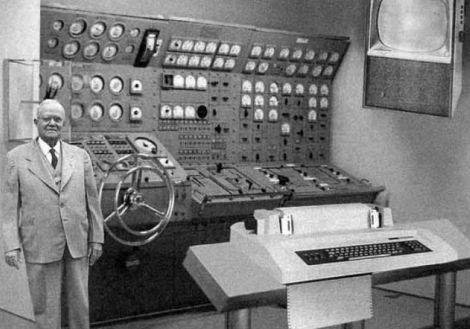
\includegraphics[height=4cm]{Old-Server.jpg}
    \end{frame}
 
 
     \begin{frame}
     	\frametitle{Corba Issues}
     	\begin{description}
     		\item[Location transparency]
     		Objects residing in the same address space and accessible with a simple function call are treated the same as objects residing elsewhere. This makes all object access as complex as the most complex case
     		
     		\item[Design and process deficiencies]
     		The creation of the CORBA standard is also often cited for its process of design by committee. There was no process to arbitrate between conflicting proposals or to decide on the hierarchy of problems to tackle. This made the specification complex, expensive to implement entirely, and often ambiguous.
     		
     	
     		
     	\end{description}
     
     \end{frame}
     \begin{frame}
     	\frametitle{Corba Issues}
     	\begin{description}	
     		\item[Problems with implementations]
     		Through its history, CORBA has been plagued by shortcomings in poor ORB implementations. 
     		\item[Firewalls]
     		CORBA (more precisely, GIOP) is not tied to any particular communications transport. 
     		If the client is behind a very restrictive firewall or transparent proxy server environment that only allows HTTP connections to the outside through port 80, communication may be impossible.
     		Recent CORBA implementations, though, support SSL and can be easily configured to work on a single port.
     		
     	\end{description}
     	
     \end{frame} 
 
    \begin{frame}
    	\frametitle{Basic Architecture}
    	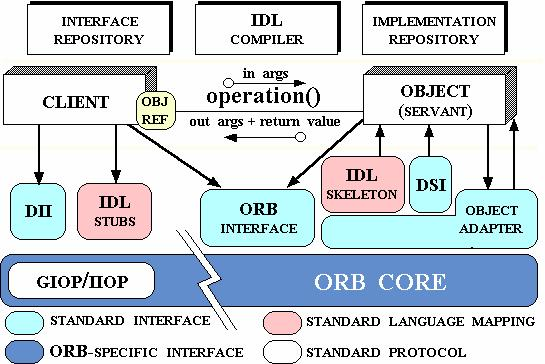
\includegraphics[height=6.5cm]{corbaArchitecture.jpeg}
    \end{frame}
       
 
    \begin{frame}
    	\frametitle{Components}
    	\begin{description}
    		\item[DII] 	Dynamic Invocation Interface allows programs to interogate object interfaces at Run-Time and generate calls
    		\item[DSI] Dynamic Server Interface. Server side version of DII where all Dynamic Invocations are received and dealth with

    		\item[Intereface Repository] 	Database of all known defined interfaces. Used by DII
    		\item[Implementation Repository] Database of all server implementations of interfaces
    		
    	\end{description}
    	
    \end{frame}           
    \begin{frame}
    	\frametitle{Components}
    	\begin{description}
    		\item[ORB] 	Object Request Broker through which all communication is channeled. Different for each implementation BUT...
    		\item[ORB Interface] Standard interface that must be implemented by all ORBs 
    		\item[GIOP] 	General Inter Object Protocol which defines how objects interact with ORB
    		\item[IIOP] 	Internet Inter Object Protocol (nuff said)
    		
    	\end{description}
    	
    \end{frame}            
    \begin{frame}
    	\frametitle{Corba Services Part I}
    	\begin{description}
    		\item[Security] 	includes security models and interfaces for application development, security administration, and the implementation of security services themselves
    		\item[Naming] 	defines how CORBA objects can have friendly symbolic names
    		\item[Events] 	decouples the communication between distributed objects (e.g. asynchronous communication)
    		\item[Relationships] 	provides arbitrary typed n-ary relationships between CORBA objects
    		\item[Externalization] 	coordinates the transformation of CORBA objects to and from external media

    	\end{description}

    \end{frame}
    
        \begin{frame}
        	\frametitle{Corba Services Part II}
        	\begin{description}
		        \item[Transactions] 	Allows use of transactions (e.g. as seen in DBMS)
        		\item[Concurrency Control] 	provides a locking service for CORBA objects in order to ensure serializable access
        		\item[Property] 	supports the association of name-value pairs with CORBA objects
        		\item[Trader] 	supports the finding of CORBA objects based on properties describing the service offered by the object
        		\item[Query] 	supports queries on objects
        	\end{description}
        
        \end{frame}
             \begin{frame}
             	\frametitle{IDL Compiler}
             	\begin{itemize}
             		\item Interface Definition Langauge defines object interfaces in language agnostic way
             		\item There exist mappings that translate IDL into Java, C, C++14, Python, ADA, and so on
             		\item Compilers exist that will translate IDL file into client and server Corba enabled code in any language
             		\item generates IDL stubs for client wishing to use object
             		\item produces IDL Skeleton for server where object is implemented
             	\end{itemize}
             	
             \end{frame}     

\end{document}

